\documentclass{article}

\usepackage{float}
% \usepackage{floatrow}
\usepackage[english, serbian c]{babel}
\usepackage[utf8]{inputenc}
\usepackage[T2A]{fontenc}
\usepackage[colorlinks=true, allcolors=blue]{hyperref}

\usepackage[a4paper, total={6in, 8in}]{geometry}

% Useful packages
\usepackage{amsmath}
\usepackage{graphicx}

\title{\Huge{Приватност и влада}\\
{\large{Семинарски рад у оквиру курса\\Рачунарство и друштво \\
        Математички факултет у Београду}}}
\author{Јован Стаменковић, 148/2017\\mi17148@alas.matf.bg.ac.rs}
\date{април 2022.}
\begin{document}
\maketitle

\tableofcontents

\newpage
\section{Увод}

Ричард Никсон је једном приликом изјавио да систем који не успе да испоштује права на приватност својих грађана, не поштује ни те грађане. Како то систем угрожава права на приватност? Какве везе имају влада, њихове службе и грађани?
\\\\
Да бисмо разумели причу морамо да се упознамо са терминима.

\begin{itemize}
  \item \textbf{Сакупљање информација} се односи на активности сакупљања личних података. Дискутоваћемо о прикупљању информација од стране владе.
  \item \textbf{Обрада информација} се односи на активности које чувају, манипулишу и користе личне податке који су сакупљени.
  \item \textbf{Ширење информација} се односи на све активности које шире личне податке. Видећемо пример закона који је дизајниран да спречи ширење информација од стране приватних организација, као и легалне начине преко којих могу да се шире информације које влада поседује.
  \item \textbf{Инвазија} се односи на активности које задиру у приватни живот особе, ометају је, или утичу на прављење одлукa. Видећемо на који начин је покушано да се ограничи инвазија.
\end{itemize}

\subsection{Догађаји који су утицали на доношење неких закона}

Први догађај, који је привукао пажњу јавности довољно да утиче на појаву закона о чувању приватних информација возача, је убиство глумице Ребеке Шафер. Једног јутра је отворила врата свог стана и упуцао ју је опседнути фан Робер Бардо. Наиме, он је њену кућну адресу сазнао преко приватног детектива који је купио информацију од одељења за моторна возила у Калифорнији. Та информација се налазила на њеној возачкој дозволи. Конгрес је након овог случаја донео закон о чувању приватних информација возача. Забрањује се откривање личних информација возача.
\\\\
Други случај, који је утицао на појаву закона о дељењу информација о регистрованим сексуалним преступницима, је случај седмогодишње Меган Канке из Њу Џерсија која је била отета, силована и затим убијена од стране комшије који је имао криминални досије као педофил. Конгрес је усвојио закон да локална полиција мора да подели информације о регистрованим сексуалним преступницима који живе у тој заједници.
\\\\
Након напада терориста 11. септембра 2001. године подигла се забринутост око безбедности. Анкета, која је направљена 2006. године, показала је да велика већина грађана (70\%) подржава повећан надзор преко камера на улицама и на јавним местима. Увођење закона који подразумева праћење интернет дискусија у собама за ћаскање и других форума подржава 62\% грађана. Ближе праћење банкарских и кредитних картица и трансакција како би се ушло у траг изворима финансирања подржава 61\% грађана. Чак је 52\% људи гласало за повећан надзор мобилних телефона и мејлова.

\newpage
\section{Тајни државни надзор}
На које начине америчка влада прикупља информације у циљу откривања и хапшења осумњичених криминалаца или зарад побољшања националне безбедности? Да ли особе увек морају да се обавесте пре почетка надзора? Одговор је не. Када се сумња на неке особе да су починиле неко кривично дело, оне не морају бити упозорене нити је потребно да се тражи дозвола пре почетка надзора.
\\\\
Поставља се питање да ли прикривени надзор крши неко од права грађана? \\
Ово питање је везано за 4. амандман. Он каже да је право човека да буде сигуран у својој кући, папирима, у својим деловањима од неоснованих претреса и заплена. Тј. да никакви налози неће бити издати за претресање. Међутим, уколико постоји нека разумна сумња која је поткрепљена потврдом или заклетвом тада ће се све испитати, тј. биће издати налози за претрес и одузимање ствари.
\begin{figure}[h!]
\centering
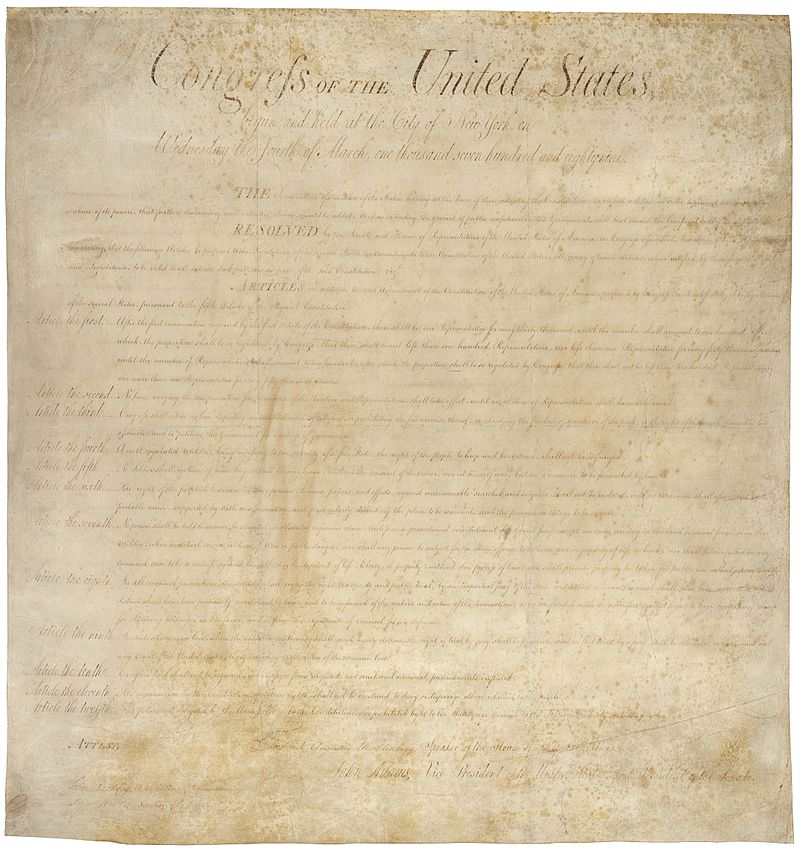
\includegraphics[width=0.6\textwidth]{Bill_of_Rights_Pg1of1_AC.jpg}
\caption{\label{fig:sangaj}Повеља о правима}
\end{figure} 

Пре америчке револуције, енглески агенти у потрази за шверцерима су користили налоге за помоћ. То им је давало овлашћење да уђу у било коју кућу или зграду и заплене сву робу коју су могли да нађу. \\

\subsection{Прислушкивање и бубице}

Прислушкивање телефона је почело још 1890-их година када су телефони почели интезивније да се користе. Држава Њујорк је 1892. године прогласила прислушкивање кривичним делом, међутим полиција у Њујорку је то игнорисала и наставила са праксом прислушкивања. До 1920. године њујоршка полиција је слушала разговоре између адвоката и клијената, лекара и пацијената, свештеника и покајника, разговоре гостију унутар хотела и тако даље.
\\\\
Прислушкивање је било популарно средство за хватање кријумчара. Најпознатији случај се односио на Роја Олмстеда који је водио посао кријумчарења вредан 2 милиона долара годишње у Сијетлу у Вашингтону. Без налога, федерални агенти су прислушкивали Олмстедов телефон и прикупили су довољно доказа да га осуде. Иако је прислушкивање било незаконито по закону Вашингтона, државни суд је признао прибављене доказе преко прислушкивања. Олмстед је апеловао све до врховног суда САД. Његов адвокат је тврдио да је полиција прекршила Олмстедово право на приватност слушањем његових телефонских разговора. Такође је тврдио да докази треба да буду одбачени јер су добијени без налога за претрес. Одлука је била 5 према 4 против Олмстеда. Образложење је било да 4. амандман штити материјалну имовину. Савезни агенти нису претресли физичко место, нису запленили физичке предмете. Тако да 4. амандман није прекршен.
\\\\
Јавност и штампа били су критични према одлуци Врховног суда. Пошто је Суд пресудио да је прислушкивање уставно, они који су се залагали за забрану прислушкивања усмерили су своје напоре на грану законодавства. 1934. године амерички Конгрес је усвојио закон који је учинио незаконитим пресретање и откривање жичане комуникације. Три године касније Врховни суд је користио Савезни закон о комуникацијама да преокрене свој став о прислушкивању без налога. У предмету Нардон против Сједињених Држава, Суд је одлучио су докази прикупљени прислушкивањем без налога били неприхватљиви. У другој одлуци, Вајс против Сједињених Држава, пресудио је да забрана прислушкивања која се примењује на унутардржавне, важи и за међудржавне телефонске разговоре. Након тога, државни тужилац је саопштио да је ФБИ прекинуо прислушкивање.
\\\\
ФБИ наравно није прекинуо прислушкивање, већ је почео да користи другачији систем за чување фајлова. Постојале су 2 врсте фајлова. Официјални фајлови који су прикупљени на легалан начин, и они тајни који су били прикупљени на нелегалан начин. На суду су се користили само официјални фајлови.
\\\\
Бубица је, као што сви знамо, скривени микрофон који се користи за надзор. Врховни суд је дошао до одлуке да грађани треба да буду заштићени и од сваког електронског надзора спроведеног без налога, укључујући и бубице. Кључна одлука је била донета 1967. године. Наиме, Чарлс Кац је користио јавни телефон за клађење. ФБИ је поставио бубицу на спољашњу страну телефонске говорнице да би се снимили Кацови телефонски разговори. Са овим доказима, Кац је осуђен због илегалног коцкања. Министарство правде је тврдило да пошто је микрофон био постављен са спољне стране телефонске говорнице, није упадао у простор који заузима Кац. У предмету Чарлс Кац против Америке, врховни суд је пресудио у корист Каца. Судија је образложио да 4. амандман штити људе, а не места. Кац је ушао у телефонску говорницу са разумним очекивањем да ће његов разговор бити приватан.
 
% \newpage
\section{Data mining - Обрада информација}
\textit{Data mining (рударење информација)} је процес претраживања једне или више база података и тражење образаца или односа међу подацима. Видећемо неколико познатих пројеката рударења података које воде владине агенције, такође видећемо и како могу настати штете када се на основу података, због алгоритама, створе погрешни профили појединаца.
\\\\
Да би се идентификовали порески обвезници који су платили мање пореза него што дугују, Пореска управа користи компјутерско упаривање и стратегије рударења. Упоређују се информације на пореском обрасцу са информацијама које обезбеђују послодавци и финансијске институције. Ово је директан начин да се открију непријављени приходи. Пореска управа сваке године ревидира неколико милиона пореских пријава. Њен циљ је да изабере поврате који највише обећавају, тј. оне који садрже грешке које резултирају тиме да није плаћен порез. Пореска управа користи алгоритам који се зове дискриминантна функција (ДИФ) за бодовање сваке пореске пријаве. ДИФ резултат је показатељ колико неправилности има на пореском обрасцу, у поређењу са пажљиво конструисаним тачним пореским пријавама. Око 60\% пореских пријава које Пореска управа ревидира јесу оне које имају висок ДИФ резултат.
\\\\
Још једна примена рударења података од стране владе је заштита друштва од непосредне опасности. Систем за надзор болести је компјутеризовани систем који анализира позиве полицији, посете хитној помоћи, изостанке из школе, куповине лекова који се издају на рецепт, и интернет претраживања како би се пронашли обрасци који би могли указују на почетак епидемије, еколошки проблем који доводи до болести или биотероризам. У јесен 2002. године систем за надзор синдрома у Њујорку, открио је пораст броја људи који траже лечење због повраћања и дијареје. Ови симптоми су били први знаци избијања Норволк типа вируса. Упозорење које је генерисао систем омогућило је градским званичницима да упозоре лекаре о појави тог вируса и саветују им да буду посебно опрезни при руковању високо заразним телесним течностима њихових пацијената.
\\\\
После 11. септембра 2001. године неколико великих телекомуникационих провајдера почело да води евиденцију телефонских разговора десетина милиона американаца Агенцији за националну безбедност (НСА), без судског налога. НСА није пратила нити снимала разговоре, већ уместо тога, анализирала је обрасце позивања у циљу откривања потенцијалне терористичке мреже. Када се касније сазнало за овај пројекат, грађани су поднели више десетина групних тужби против телекомуникационих компанија.
\\\\
Стручњаци су почели да упозоравају на личне штете које могу настати када организације делују на основу индивидуалних профила који су конструисани преко рударења информација. Једна компанија је преко рударења предвиђала које су жене трудне, како би могли да им директно шаљу понуде за ствари које користе труднице. Тако је једном компанија послала огласе за одећу за труднице и дечији намештај тинејџерки пре него што је она рекла оцу да је трудна.
Имамо други пример где владина агенција користи податке да профилише људе и процени ко може бити потенцијални терориста. Шта се дешава ако сви ти компликовани алгоритми погрешно профилишу некога, и невиног човека ставе на листу за потенцијалне терористе? Толико су компликовани алгоритми као и количина података којим они располажу да ниједан човек не може да објасни зашто је некога алгоритам профилисао као потенцијалног терористу. Постоји више милиона имена у САД који се налазе на тој листи за потенцијалне терористе, а десетине хиљада људи са тог списка се нађу и на списку за забрану летења.

\newpage
\section{Ширење информација}

На шта се односи Закон о слободи информација? То је закон који је осмишљен да промовише отвореност влада, дозвољавајући новинским организацијама и приватним грађанима да приступе информацијама које имају федералне агенције. Такође, видећемо како се информације које је прикупила влада за једну сврху, наплату путарине, користе као доказ о томе где се људи налазе у случају злочина или неког грађанског случаја.
\\\\
\textbf{Закони о ширењу информација}:
\begin{itemize}
  \item Закон о правима на породично образовање и приватност обезбеђује ученицима који имају 18 и више година право на увид у своју образовну евиденцију и да имају право да захтевају измене записа који садрже погрешне податке. Ученици такође имају право да спрече ширење информација о њима без њихове дозволе, осим под одређеним околностима. За ученике млађе од 18 година ова права имају њихови родитељи или старатељи. Овај закон се односи на све образовне установе које добијају средства од министарства образовања САД.
  \item 1988. председник Роналд Реган је предложио судију Роберта Борка за Врховни суд САД-а. Борк је био истакнути конзервативац и
  његова номинација је била контроверзна. Видеотека у Вашингтону доставила је листу Боркових изнајмљених видео записа репортеру који је радио за Вашингтон Сити пејпер. Тај лист је затим објавио листу. Док је намера највероватније била да се осрамоти Борк, тај чланак је имао и ефекат да се донесе нови закон о заштити приватности видео записа 1988. године. Према овом закону, видео провајдери (укључујући провајдере онлајн снимака) не могу откривати записе о изнајмљивању без писмене сагласности купца. Поред тога, организације морају уништити личне податке о закупу у року од годину дана од датума када су ове информације престале да буду битне за сврху због које су прикупљене.
  \item Овај закон се односи на заштиту приватности пацијената. Ове смернице ограничавају како лекари, болнице, апотеке и осигуравајућа друштва могу користити информације прикупљене од пацијената. Прописи покушавају да ограниче размену информација међу пружаоцима здравствених услуга и да се размењују само оне информације које су неопходне за бригу о пацијенту. Забрањује се здравственим радницима да дају информације компанијама за животно осигурање, банкама или другим предузећима без посебног потписа тј. овлашћења од лица које се лечи.
  \item Закон о слободи информација је закон који је осмишљен да осигура да јавност има приступ евиденцији америчке владе. Међутим, овај закон носи претпоставку да ће влада пустити тражене информације у јавност. Ако агенција не открије информације, мора објаснити зашто се те информације чувају. Постоји девет изузетака у Закону о слободи информација, тј. оне ситуације у којима влада може легитимно да одустане од пуштања информација. На пример, документ може бити задржан ако је класификован као тајна због националне одбране или спољне политике. Такође, влада може ускратити објављивање докумената који садрже тајне што се тичу трговине или неке поверљиве комерцијалне или финансијске информације. Такође, изузеће се односи и на документе који се односе на спровођење закона истраге.
\end{itemize}

\newpage
\subsection{Информације скупљене на наплатним рампама и суд}
E-ZPass је аутоматски систем наплате путарине који се користи на већини путева са наплатом путарине као што су мостови и тунели између Иланоја и Мејна. Возачи који имају инсталирану E-ZPass ознаку у својим возилима, могу да прођу кроз наплатне рампе без заустављања да се физички плати путарина. Уместо тога, E-ZPass читач инсталиран у аутоматизованој наплатној траци добија информације од ознака аутомобила који пролазе и скида одређену своту новца са рачуна сваког возача. 
\\\\
Министарство саобраћаја државе Њујорк има инсталиране читаче ознака на локацијама које нису наплатне станице ради праћења напредовања појединих возила. На овај начин систем може да обезбеди корисне информације другим возачима приказивањем на електронским знаковима процењено време за долазак до популарних дестинација. Према министарству, систем шифрује информације са појединачне ознаке, брише информације чим возило прође последњи читач, и никада не чини доступним информације о појединачним возилима.
\\\\
Државе користе информације прикупљене на овај начин у судским процесима. Добро познат пример је случај Мелани МекГвајер, медицинске сестре из Њу Џерсија која је била осумњичена да је убила свог мужа и бацила његов раскомадан леш у воду. Да би им помогли да докажу свој случај против Мелани, тужиоци су користили E-ZPass записе да реконструишу њено кретање. 

\newpage
\section{Инвазија}
Живимо у времену када људи све чешће морају уступити приступ њиховим личним подацима ако желе да користе неку услугу. То се одражава на приватност. Уколико неко или нешто омета приватност људи или утиче на доношење неке одлуке, то се сматра инвазијом приватности. Видећемо два примера владиних акција за спречавање инвазије, а затим две владине акције које се могу сматрати инвазивним.

\subsection{Владине акције за спречавање инвазије}
У Америци је велики део становништва негодовао јер су их у време вечере звали продавци да им нуде производе. То се сматрало узнемиравајућом инвазијом на приватност. Све више њих се изјашњавало да им таква узнемиравања сметају. Као покушај решења направили су "Не зови"  регистар. То је бесплатна услуга која омогућава људима који не желе да примају позиве, да региструју своје бројеве телефона. Јавност је била одушевљена и регистровали су преко 50 милиона бројева телефона пре него што је тај сервис уопште и ступио на снагу у октобру 2003. године. Регистар "Не зови" није елиминисао 100\% непожељних позива. Прописи изузимају политичке организације, добротворне организације и организације које спроводе телефонске анкете. Чак иако је ваш број телефона регистрован, можда ћете и даље примати телефонске позиве од компанија са којима сте пословали у протеклих 18 месеци. Ипак, очекује се да ће регистар спречити већину продаваца да зову људе који не желе да примају позиве. Корист од заштите људи од тих позива се процењује да је већа него штета која је проузрокована постављењем ограничења за телефонско оглашавање.
\\\\
Шездесетих година прошлог века телевизијски гледаоци су се жалили федералној комисији за комуникације због гласних реклама. Барак Обама је потписао закон о ублажавању гласноће комерцијалних огласа 2010. године. Тај закон је захтевао да се обезбеди да телевизије пуштају рекламе истом јачином као што су били програми који су прекинути. Представница спонзора овог закона Ана Есхо је рекла да су потрошачи тражили решење за овај проблем деценијама, а да га данас коначно имају. И да је то једноставно решење за велики проблем.

\subsection{Владине акције које су инвазивне}
У настојању да се обузда нелегална производња метамфетамина, савезне и државне владе донеле су законе којима се ограничава куповина производа који садрже псеудоефедрин, који се користи у производњи метамфетамина. Закон о борби против епидемије метамфетамина ограничава количину псеудоефедрина коју појединац може да купи на месечном нивоу. Питање је да ли су закони били делотворни. У већини држава, оригинални псеудоефедрин се и даље продаје иза тезге одраслима. Међутим, сви морају показати личну карту и попунити дневник продаје својим именом, адресом и потписом. Две државе, Орегон и Мисисипи захтевају рецепт за куповину производа који садржи псеудоефедрин. У неколико објављених случајева, баке и деке који су куповале лекове против прехладе за чланове своје породице били су ухапшени јер су прекорачили ограничење за куповину псеудоефедрина.
\\\\
У настојању да обезбеди већу безбедност путника на аеродромима, управа за безбедност саобраћаја почела је да примењује напредне скенере за прављење слика 2007. године. Неки скенери користе повратно распршивање рендгенских зрака како би се добила детаљна слика тела путника, а други скенери користе милиметарске таласе. Тестирање скенера је почело на међународном аеродрому Скај Харбор у Фениксу 2007. године. Када је први систем стављен у функцију, путници који су пали на примарним безбедоносним контролама могли су да бирају између рендгенског скенирања и традиционалне тoп-даун претраге. У јуну 2011. године управа за безбедност саобраћаја је објавила да је већ распоредила 500 скенера, и да би уз још 500 комада то покрило 60\% свих путника на аеродромима у Сједињеним државама. Док су ужурбано постављали системе, управа за безбедност саобраћаја се борила против критичара. Неки људи су били увређени због слика које су произвели скенери јер откривају све анатомске карактеристике. Електронски информативни центар о приватности поднео је тужбу за суспензију скенер система. Центар је овај програм назвао незаконитим, инвазивним и неефикасним, тврдећи да је прекршио закон о приватности, закон о слободи вероисповести и четврти амандман. 2011. године управа за безбедност саобраћаја је објавила да се спрема тестирање новог софтвера за напредно снимање. Из управе су рекли да нови систем аутоматски детектује потенцијалне претње и указује на њихову локацију на општем прегледу особа. Тестови су били успешни, а у јануару 2013. године објављено је да ће сви они скенери који праве слике специфичне за путнике бити уклоњени са аеродромских контролних пунктова до јуна 2013. године.

\begin{figure}[h!]
\centering
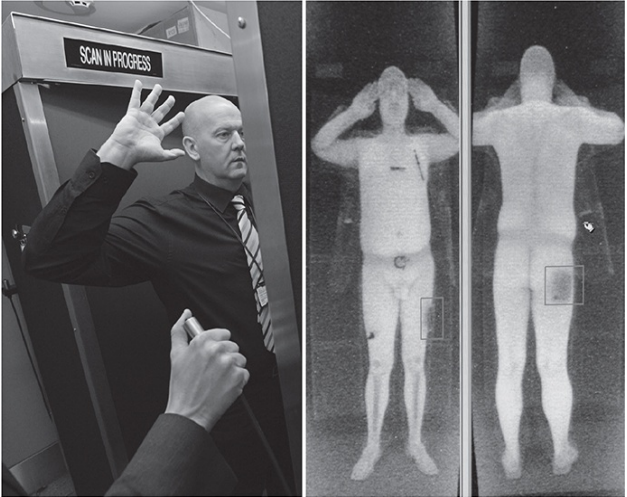
\includegraphics[width=0.6\textwidth]{PrimerSkenera.png}
\caption{\label{fig:sangaj}Пример рада скенера}
\end{figure} 

\section{Закључак}
Видели смо начине на које влада скупља, обрађује и користи информације и на законит и на незаконит начин. Кажу да је то све за добробит грађана, а да ли је заправо тако?
\\\\
Сматрам да влада превише завирује у приватност грађана и да би требало да се некако ограничи. Наравано, неки систем треба да постоји, али тако да не угрожава појединце.

\newpage
\section{Литература}
\bibliographystyle{alpha}
\bibliography{bibliography} 
[1] Ethics for the Information Age, 7th Edition by Michael J. Quinn (z-lib.org). 
[2] https://www.uscourts.gov/about-federal-courts/educational-resources/about-educational-outreach/activity-resources/what-does-0

\begin{thebibliography}{9}
			
			\bibitem{prva}
			Ethics for the Information Age, 7th Edition by Michael J. Quinn (z-lib.org). 
			\bibitem{fourth amendment}
			\href{https://www.uscourts.gov/about-federal-courts/educational-resources/about-educational-outreach/activity-resources/what-does-0}{https://www.uscourts.gov/about-federal-courts/educational-resources/about-educational-outreach/activity-resources/what-does-0}
			\bibitem{rebecca}
			\href {https://reelreviews.com/shorttakes-56/rebecca-schaeffer/rebecca-schaeffer}{https://reelreviews.com/shorttakes-56/rebecca-schaeffer/rebecca-schaeffer}
			\bibitem{megan}
			\href {https://www.aetv.com/real-crime/megans-law-story}{https://www.aetv.com/real-crime/megans-law-story}
			\bibitem{roy}
			\href {https://www.historylink.org/file/4015}{https://www.historylink.org/file/4015}
			\bibitem{megan}
			\href {https://us.norton.com/blog/privacy/do-not-call-registry#}{https://us.norton.com/blog/privacy/do-not-call-registry#}
			
		\end{thebibliography}


\end{document}
